\section{Method}

\label{sec:method}

The controlled evaluation design holds the candidate bank, packing policy, metadata, token budgets, answering model, and memory wrapper fixed across all selectors. Only the scoring function that orders candidates changes. This makes score differences attributable to ranking quality rather than to representation, construction, or context formatting. The Baseline Selectors subsection describes the existing selectors against which CTLS is compared. The CTLS subsection introduces CTLS as the principled corrective algorithm. The Protocol subsection gives the evaluation protocol shared by all selectors.


\begin{figure}[htbp]
\centering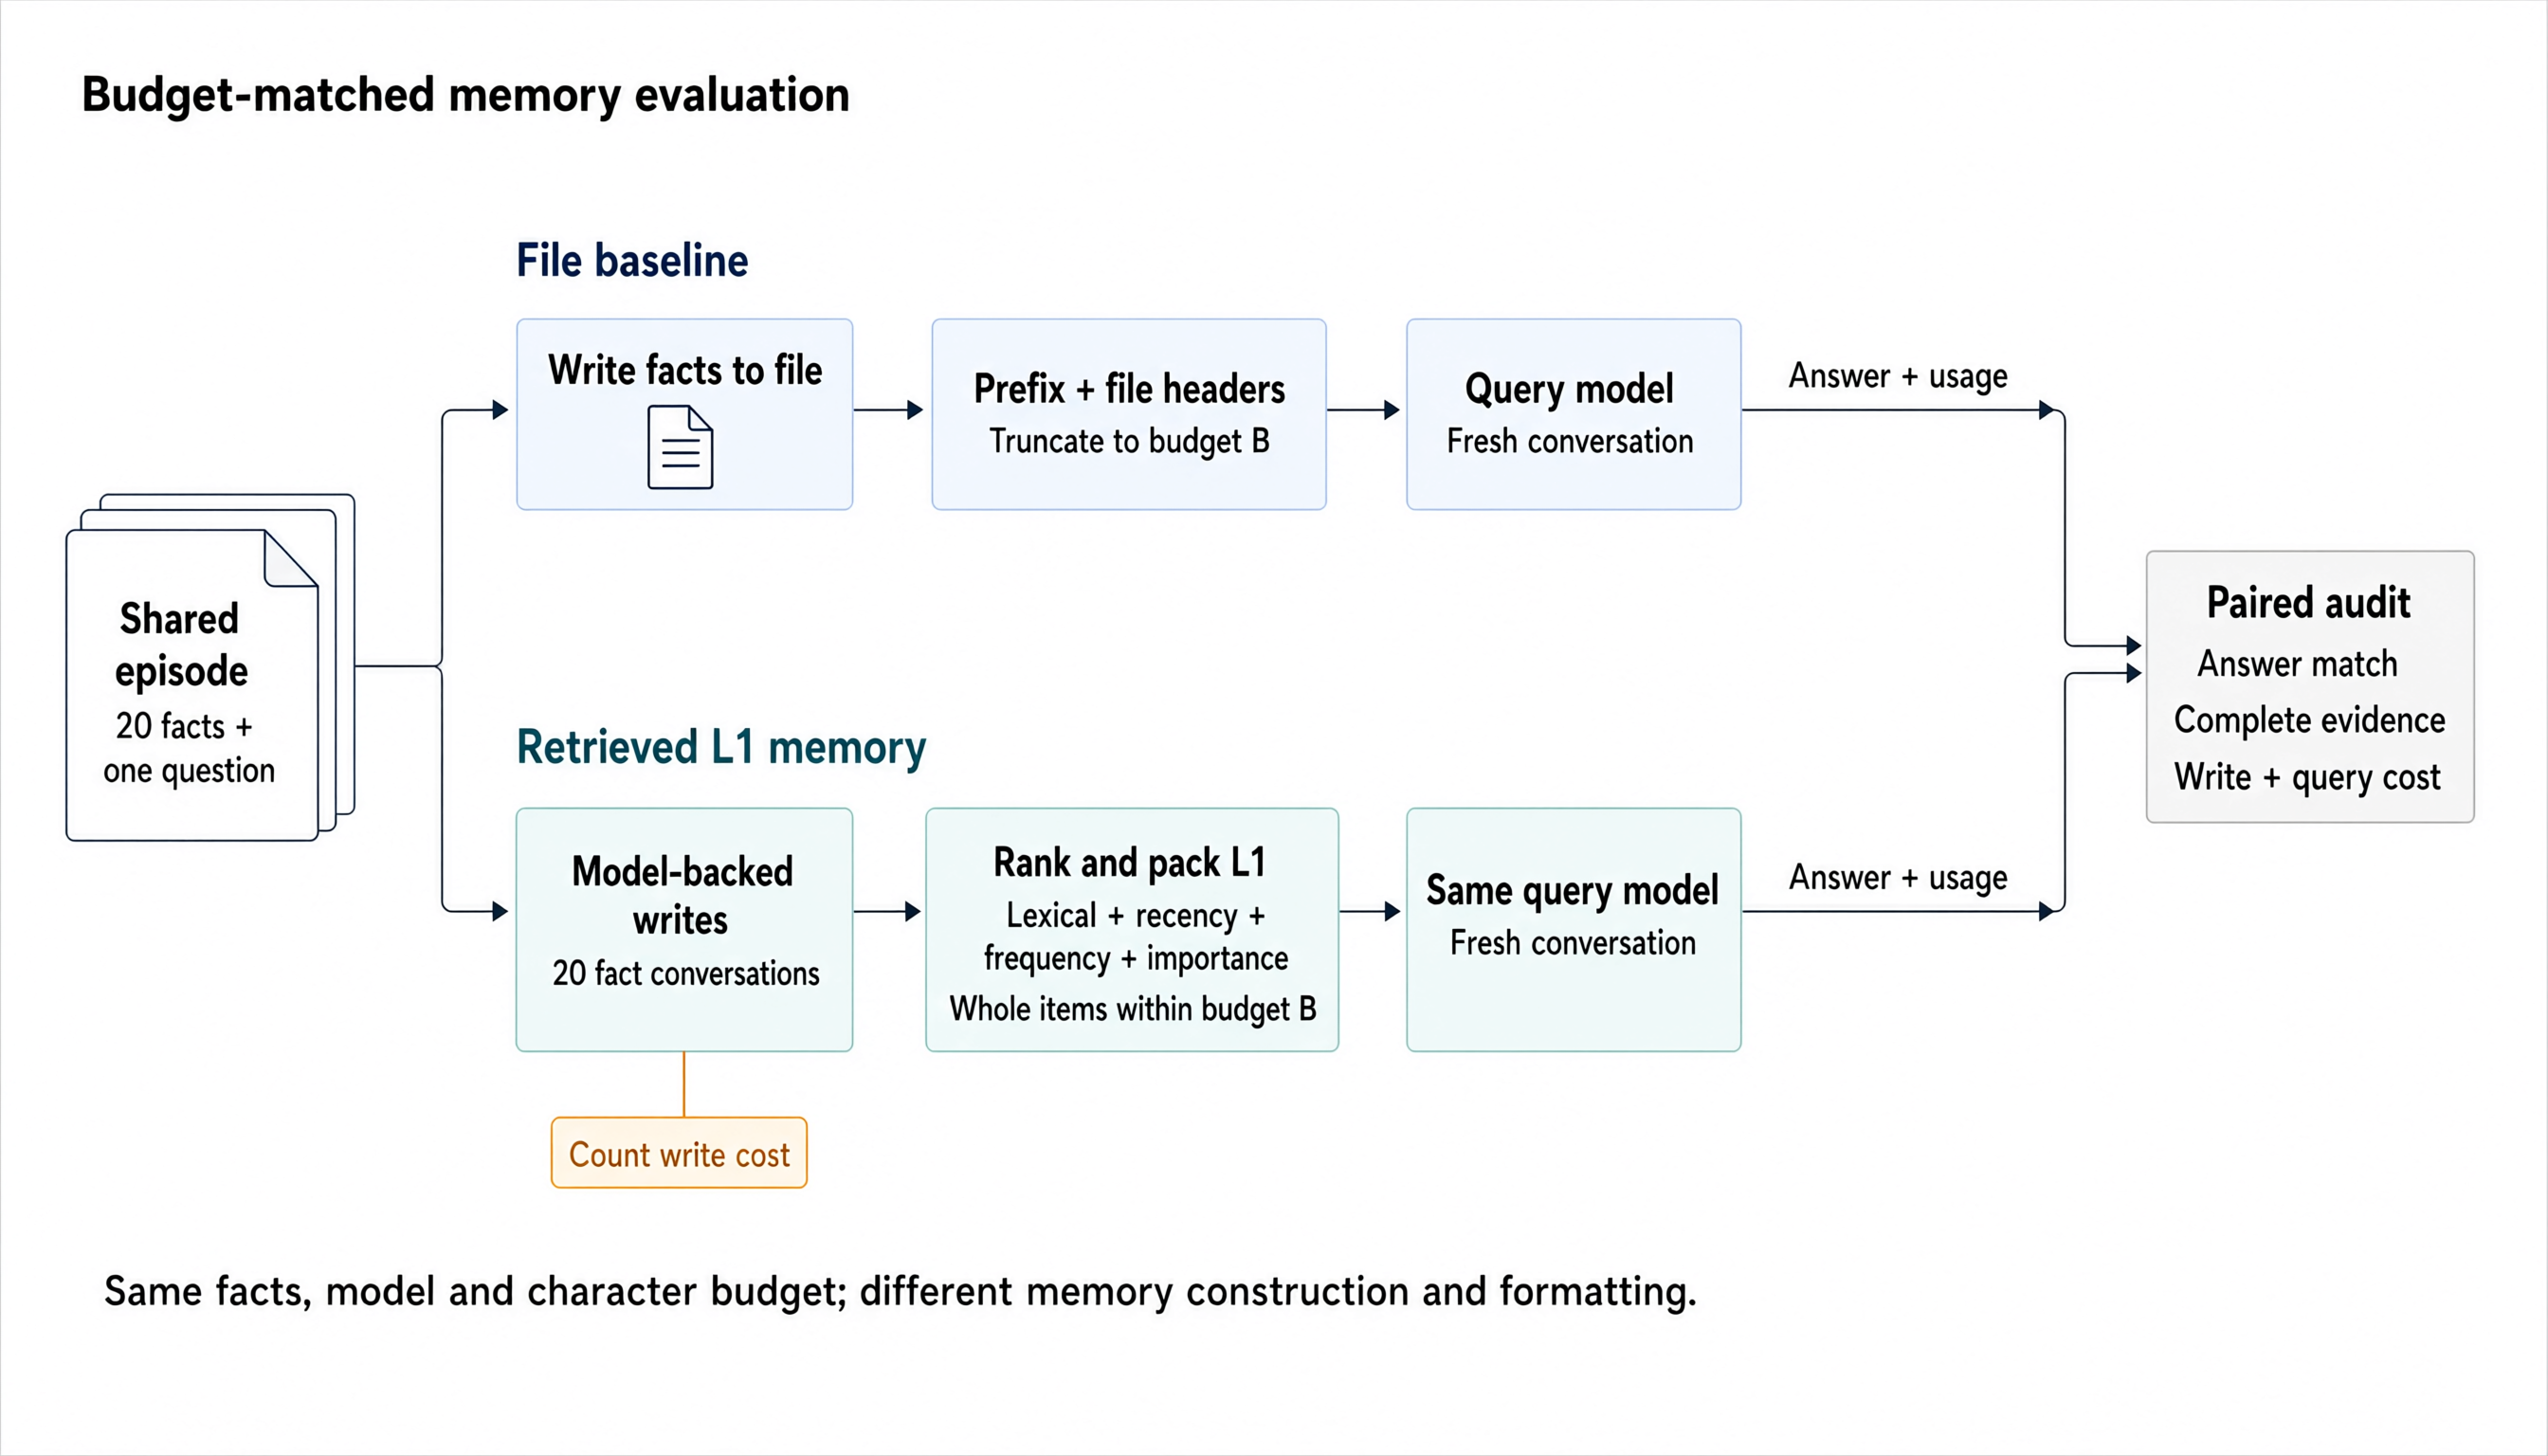
\includegraphics[width=\linewidth]{figures/methodology.png}
\caption{Budget-matched evaluation of two operational memory paths. The retrieved arm
incurs model-backed write cost before its isolated query. Equal character caps include
each arm's own formatting overhead. This schematic illustrates the audited implementation;
it is not an experimental result.}
\label{fig:methodology}\end{figure}
\subsection{Frozen Memory and Matched Token Packing}

\label{sec:method_baseline}

The baseline selectors operate on a frozen single-layer bank: complete source histories retained in their original form, segmented losslessly into turn segments bounded by a pinned Qwen3 BPE tokenizer. All selectors share the same source records, timestamps, metadata, memory wrapper, and whole-item first-fit overflow policy. The prefix selector uses bank order with no scoring. The recency selector keeps only the temporal decay term. The Jaccard selector keeps only lexical overlap over lowercased alphanumeric token sets. The deployed hybrid combines all four terms with fixed weights: lexical Jaccard overlap, temporal decay, bounded log-frequency, and heuristic importance. The hybrid\_no\_time ablation sets the temporal weight to zero and renormalizes remaining weights so lexical overlap retains proportional dominance. BM25 uses a standard probabilistic lexical score with positive inverse document frequency. The primary comparison is BM25 against the deployed hybrid.

The controlled comparison holds all variables fixed across arms: question identifiers, answering model and version, decoding settings, system prompt, canonical memory items, memory wrapper, tokenizer, packing policy, and write path. Only the selector scoring function changes. Frequency is held at a fixed value and importance at a fixed value across all selectors so that hybrid\_no\_time and Jaccard coincide as a sanity equivalence check, confirming that any remaining gap between the deployed hybrid and BM25 is attributable to the temporal term rather than to frequency or importance variation.

\subsection{Contrastive Tier-Based Lexical Selection (CTLS)}

\label{sec:method_ctls}

CTLS (Contrastive Tier-Based Lexical Selection) is a novel selector that partitions candidates into a lexically relevant tier (Jaccard overlap strictly positive) and a lexically absent tier (Jaccard overlap equal to zero) before applying any temporal scoring. Within the relevant tier, candidates are ranked by the full hybrid score so temporal decay and frequency serve as tiebreakers among genuinely relevant items. Within the absent tier, recency plus importance provides fallback ordering. Packing draws from the relevant tier first in descending score order, then from the absent tier in descending recency order, using the same whole-item first-fit policy as all other selectors. \citep{ref_959d6858d034c6e1}

The Non-Dominance Property follows directly from the tier partition. For any candidate with positive overlap and any candidate with zero overlap, CTLS places the positive-overlap item in the relevant tier and the zero-overlap item in the absent tier. Since packing exhausts the relevant tier entirely before inserting any absent-tier item, the relevant item is always considered for inclusion first, regardless of temporal decay, frequency, importance, or any weight values. No assignment of weights to temporal, frequency, or importance terms can cause an absent-tier item to displace a relevant-tier item. This eliminates temporal dominance by construction. CTLS requires no model calls, no embedding model, and no learned parameters. It is a zero-cost selector substitution compatible with the existing write path, packing policy, and memory wrapper. \citep{ref_ab2c226739f2f52a}

The relationship between CTLS and hybrid\_no\_time clarifies within-tier temporal ordering. hybrid\_no\_time discards temporal information entirely by setting the temporal weight to zero globally. CTLS preserves temporal decay as a within-tier tiebreaker: for two relevant-tier candidates with identical Jaccard scores, the temporal decay term breaks the tie. For queries where every candidate has positive overlap, CTLS and hybrid\_no\_time produce identical rankings when non-temporal terms are also equal, but CTLS retains recency information for cases where they differ. For mixed-tier queries -- the typical case for short questions against long conversational segments -- CTLS provably outperforms hybrid\_no\_time by guaranteeing relevant-tier priority. The hybrid\_no\_time empirical result is therefore a conservative lower bound on the improvement from CTLS.

\subsection{Repeated Real Agent Evaluation and Ablation Design}

\label{sec:method_protocol}

Each memory episode has its own fact set and fresh agent instances. The frozen bank design holds source records, timestamps, metadata, and segment content fixed across all selectors; write tokens are zero and construction cost is identical across every arm. The formal question uses a new conversation ID so that no seeding dialogue leaks into the query context. The runner verifies isolated query history and confirms actual memory injection before scoring. \citep{ref_ab2c226739f2f52a}

Evidence recall requires the complete annotated turn to appear in the delivered context; evidence-session recall requires any segment from the annotated session to be selected. Three answering calls per memory episode are averaged before stratified cluster bootstrap inference with Holm correction across all prespecified comparisons. The pinned original LongMemEval task-specific grading prompts are evaluated with a fixed primary judge model; strict yes/no parsing and arm-blind response keys replace substring grading. A second fixed model audits a deterministic sample. The evaluation adapts the stratified extraction paradigm of LongMemEval; the resulting subset is not an official benchmark score. Blinded human adjudication of model disagreements remains an open task before final paper submission.

\FloatBarrier

\subsection{Formal Analysis: Temporal Dominance and the Non-Dominance Property}
\label{sec:method_formal}

We now formalize temporal dominance and state the Non-Dominance Property that CTLS satisfies by construction.

\begin{definition}[Scoring function]
Let $q$ be a query and $m$ a memory candidate. The deployed hybrid scoring function is
\begin{equation}
  s_{\mathrm{hyb}}(q,m) = w_s J(T(q),T(m)) + w_t D(m) + w_f F(m) + w_i I(m),
  \label{eq:hybrid}
\end{equation}
where $J(A,B)=|A\cap B|/|A\cup B|$ is Jaccard overlap between lowercased token sets; $D(m)=2^{-a(m)/h}$ is exponential temporal decay with half-life $h$; $F(m)=\min\{\log(1+f(m))/\log(101),1\}$ is bounded log-frequency; and $I(m)$ is a heuristic importance score. The deployed weights are $w_s=0.4$, $w_t=0.3$, $w_f=0.2$, $w_i=0.1$.
\end{definition}

\begin{definition}[Temporal dominance]
Given two candidates $m_{\mathrm{old}}$ and $m_{\mathrm{fresh}}$ with $J(q,m_{\mathrm{old}}) > J(q,m_{\mathrm{fresh}})$ (the older item is more lexically relevant) and $D(m_{\mathrm{fresh}}) > D(m_{\mathrm{old}})$ (the newer item has higher temporal decay), temporal dominance occurs when the hybrid ranks $m_{\mathrm{fresh}}$ above $m_{\mathrm{old}}$:
\begin{equation}
  w_t\bigl(D(m_{\mathrm{fresh}})-D(m_{\mathrm{old}})\bigr) > w_s\bigl(J(q,m_{\mathrm{old}})-J(q,m_{\mathrm{fresh}})\bigr).
  \label{eq:dom_condition}
\end{equation}
\end{definition}

Equation~\ref{eq:dom_condition} reveals the structural vulnerability: with $w_t/w_s = 0.75$, the freshness gap needs only to be $0.75$ times the lexical advantage to flip the ranking. Because Jaccard scores between short queries and long conversational segments are typically small and concentrated near zero, moderate freshness gaps routinely satisfy this condition.

\begin{definition}[CTLS selector]
The CTLS scoring function partitions candidates into two tiers before scoring:
\begin{align}
  \mathcal{T}_0(q) &= \{m \in \mathcal{C} : J(T(q),T(m)) > 0\}, \label{eq:tier0} \\
  \mathcal{T}_1(q) &= \{m \in \mathcal{C} : J(T(q),T(m)) = 0\}. \label{eq:tier1}
\end{align}
Items in $\mathcal{T}_0$ are ranked by $s_{\mathrm{hyb}}(q,m)$ descending. Items in $\mathcal{T}_1$ are ranked by $w_t D(m) + w_i I(m)$ descending. Packing inserts items from $\mathcal{T}_0$ in ranked order until the budget $B$ is exhausted or $\mathcal{T}_0$ is drained, then inserts items from $\mathcal{T}_1$.
\end{definition}

\begin{theorem}[Non-Dominance Property]
Under CTLS, for any $m_r \in \mathcal{T}_0(q)$ and any $m_a \in \mathcal{T}_1(q)$, $m_r$ is offered to the greedy packer before $m_a$, regardless of $D(m_a)$, $F(m_a)$, $I(m_a)$, or the values of $w_t$, $w_f$, $w_i$. If $m_r$ fits within the remaining budget when it is considered, it is inserted before any tier-1 item is attempted. No tier-1 item can preempt a tier-0 item's insertion attempt.
\end{theorem}

\begin{proof}
By definition, $m_r \in \mathcal{T}_0(q)$ implies $J(T(q),T(m_r)) > 0$ and $m_a \in \mathcal{T}_1(q)$ implies $J(T(q),T(m_a)) = 0$. CTLS exhausts the entire $\mathcal{T}_0$ list before attempting any item in $\mathcal{T}_1$. Therefore $m_r$ is offered to the packer before $m_a$ regardless of their individual scores. The greedy packer applies a whole-item first-fit rule: if $m_r$ fits within the remaining budget it is inserted; if it does not fit it is skipped and the packer advances to the next $\mathcal{T}_0$ item. In neither case is any $m_a \in \mathcal{T}_1$ offered before the $\mathcal{T}_0$ list is exhausted. A budget that fills entirely with tier-0 items causes all tier-1 items to be excluded; a budget that is not exhausted by tier-0 admits tier-1 items only after all tier-0 candidates have had their insertion attempt. \qed
\end{proof}

The theorem guarantees priority ordering under the greedy first-fit packer: every tier-0 item receives its insertion attempt before any tier-1 item does. A tier-0 item that is too large to fit the remaining budget is skipped, not displaced; no tier-1 item takes its slot. The guarantee is structural and deterministic for any $w_t > 0$ and any freshness gap. Temporal dominance is eliminated by construction rather than by weight tuning.

\subsection{Adaptive Query-Conditioned Temporal Scoring}
\label{sec:method_adaptive}

The mechanism inequality (Eq.~\ref{eq:dom_condition}) reveals two actionable levers: the weight ratio $w_t/w_s$ and the half-life $h$. Rather than setting these globally, one can make $w_t$ query-conditioned:
\begin{equation}
  w_t^*(q) = w_t^{\max} \cdot \sigma\!\bigl(-\lambda\,(\bar{J}(q) - \mu)\bigr),
  \label{eq:adaptive_wt}
\end{equation}
where $\bar{J}(q) = |\mathcal{C}|^{-1}\!\sum_{m \in \mathcal{C}} J(T(q),T(m))$ is the mean lexical overlap between the query and the candidate set, $\sigma$ is the logistic function, $\mu$ is a pivot overlap level, and $\lambda > 0$ controls sensitivity. When queries are lexically specific, $w_t^*$ collapses toward zero so that relevance dominates. When queries are lexically vague, $w_t^*$ recovers toward $w_t^{\max}$, using recency as a tiebreaker. This adaptive scorer subsumes both CTLS and hybrid\_no\_time as special cases and requires only one extra pass over the candidate set with no model calls. It is a proposed extension; the current paper evaluates the tier-partition formulation of CTLS.

\subsection{Three-Level Memory Architecture}
\label{sec:method_architecture}

The controlled evaluation exercises a frozen single-layer bank, but the broader JiuwenSwarm system organizes agent memory across three layers that differ in scope, durability, and access latency.

\begin{definition}[Three-Level Memory]
Let $\mathcal{M} = (L_1, L_2, L_3)$ where each $L_k$ is a tuple $(S_k, \tau_k, \kappa_k, \pi_k)$ of storage backend, time-to-live, item capacity, and promotion policy. Layer $L_1$ is process-local; $L_2$ is session-durable; $L_3$ is project-persistent.
\end{definition}

\begin{table}[htbp]
\centering\small
\caption{Default parameters for the three memory layers. The controlled selector study evaluates a frozen read-only single-layer bank; the three-layer hierarchy is the production design.}
\label{tab:memory_layers}
\begin{tabular}{lcccl}\toprule
Layer & Backend & TTL (s) & Capacity & Scope \\\midrule
$L_1$ & In-process dict & 3600 & 20 items & Single process \\
$L_2$ & SQLite/Redis & 86400 & Unlimited & Single session \\
$L_3$ & Markdown file & None & Unlimited & Project lifetime \\
\bottomrule\end{tabular}
\end{table}

At query time, the retrieval path consults $L_1$ first. On a miss it searches $L_2$ and promotes the hit to $L_1$. $L_3$ is consulted last and yields prefix content. CTLS operates at the $L_1$ scoring step; its tier partition and Non-Dominance Property apply identically in a multi-layer setting because the partition depends only on query-candidate Jaccard overlap, not on layer membership.

\subsection{Scientific Literature Agent Pipeline}
\label{sec:method_agent}

The memory subsystem described above is exercised in isolation in the controlled evaluation, but it is embedded in a broader multi-agent pipeline designed for autonomous scientific literature processing. The pipeline addresses a concrete gap: current agent frameworks retrieve documents and answer questions, but they do not maintain a queryable record of what has been read, why it was retrieved, or how individual claims relate to a developing hypothesis. The design contributes three properties absent from standard retrieval-augmented generation pipelines.

\textbf{Role decomposition.} Four specialized agents operate in sequence:
(1)~a \emph{retriever} issues keyword and semantic queries and returns candidate documents;
(2)~a \emph{reader} extracts claims, evidence snippets, and citation links and writes each as a structured memory item to $L_2$;
(3)~a \emph{critic} scores each stored claim on relevance, novelty, and internal consistency, updating the heuristic importance score $I(m)$;
(4)~a \emph{synthesiser} draws on $L_1$ working memory to draft a section and records open questions as new retrieval seeds.

\textbf{Provenance-preserving memory items.} Each item written by the reader carries a structured provenance record: document identifier, section, page, and claim type. Provenance is stored in the metadata field alongside the importance score, making it possible for the synthesiser to trace every sentence in its output back to a source document. This is not implemented in the current controlled evaluation, which uses raw source turns without structured provenance; it is a design extension motivated by the memory architecture's per-item metadata support.

\textbf{Iterative hypothesis refinement.} After each synthesis step the critic compares the draft against the stored claims, identifies unsupported assertions, and generates targeted retrieval queries. These re-enter the retriever as next-step seeds, closing a feedback loop. The loop terminates when the critic's relevance score for marginal retrieved documents falls below a threshold, or when a maximum iteration count is reached.

\begin{figure}[htbp]
\centering
\begin{tikzpicture}[
  agent/.style={draw,rounded corners=4pt,minimum width=2.5cm,
                minimum height=0.85cm,align=center,font=\small,fill=white},
  store/.style={draw,cylinder,shape border rotate=90,aspect=0.25,
                minimum width=1.8cm,minimum height=0.7cm,
                align=center,font=\scriptsize,fill=gray!10},
  arr/.style={-{Stealth[length=5pt]},thick},
  darr/.style={arr,dashed,gray!70},
  lbl/.style={font=\scriptsize,align=center}
]
\node[agent,fill=blue!10]  (R)  at (0,0)    {Retriever};
\node[agent,fill=teal!10]  (Rd) at (3.2,0)  {Reader};
\node[agent,fill=orange!10](Cr) at (6.4,0)  {Critic};
\node[agent,fill=purple!10](Sy) at (9.6,0)  {Synthesiser};
\node[store] (mem) at (4.8,-2.0) {$L_1$/$L_2$ Memory\\(provenance items)};
\node[lbl,above=0.5cm of R] (corpus) {Corpus / API};
\draw[arr] (corpus) -- (R);
\draw[arr] (R)  -- node[above,lbl]{docs} (Rd);
\draw[arr] (Rd) -- node[above,lbl]{claims} (Cr);
\draw[arr] (Cr) -- node[above,lbl]{scored\\items} (Sy);
\draw[darr] (Rd.south) to[bend right=15] node[left,lbl]{write} (mem.north west);
\draw[darr] (mem.north east) to[bend left=15] node[right,lbl]{read} (Sy.south);
\draw[darr] (Cr.south) to[bend left=8] node[right,lbl]{update $I(m)$} (mem.east);
\draw[arr,bend right=50] (Sy.east) to node[right,lbl]{open\\queries} ++(1.2,0)
  -- ++(0,1.8) -| node[above,lbl,pos=0.25]{retrieval seeds} (R.north);
\draw[arr] (Sy.east) -- ++(1.3,0) node[right,lbl]{Draft\\section};
\end{tikzpicture}
\caption{Scientific literature agent pipeline. Four specialized agents operate in sequence; the synthesiser re-seeds retrieval with open questions, closing a feedback loop. Memory items carry provenance records in addition to the scoring metadata evaluated in the controlled study. This is a design description; the current experiments evaluate the memory retrieval component in isolation.}
\label{fig:pipeline}
\end{figure}

\FloatBarrier

\subsection{Budget-Constrained Packing as Binary Knapsack}
\label{sec:method_packing}

The whole-item first-fit packing policy used in all selectors is a deterministic greedy heuristic. An exact formulation casts item selection as a binary knapsack problem: given a set of scored candidates $\{m_1,\ldots,m_k\}$ with token lengths $\ell_i$ and relevance scores $s_i$, choose a subset $\mathcal{S} \subseteq [k]$ to maximize $\sum_{i \in \mathcal{S}} s_i$ subject to $\sum_{i \in \mathcal{S}} \ell_i \le B$. With $k \le 10$ candidates, the exact solution is tractable by exhaustive search in $O(2^k)$ time or by dynamic programming in $O(kB)$ time.

The greedy heuristic can leave budget unused when the top-ranked item is long and two shorter lower-ranked items would cover more score within the same budget. The gap between greedy and optimal is bounded by the score of the single largest item skipped, which is typically small when candidates have similar lengths. For the evaluation in this paper the packing policy is held constant across all selectors, so packing differences do not confound the comparison. Replacing the greedy packer with the exact knapsack solution is an orthogonal improvement that could be applied to any selector including CTLS; this paper does not evaluate it.

\FloatBarrier
Let $q$ be a question, $M$ its episode memory, and $B$ the cap on the entire
injected memory section, including headings and metadata. The baseline constructs
a file-derived section and keeps its prefix. The retrieved arm scores stored
exchanges, takes at most $k=10$ candidates, and greedily appends complete formatted
items that fit. An over-budget item is skipped rather than partially appended;
later smaller items can still be considered. Thus equal $B$ does not imply equal
usable fact content or identical prompt formatting.
\begin{equation}
  s(q,m)=0.4J(T(q),T(m))+0.3\,2^{-a(m)/h}
       +0.2\min\!\left\{\frac{\log(1+f(m))}{\log(101)},1\right\}+0.1I(m),
  \label{eq:ranking}
\end{equation}
where $T$ lowercases text and keeps alphanumeric/underscore word tokens longer
than one character; $J(A,C)=|A\cap C|/|A\cup C|$ (zero for an empty set);
$a(m)$ is age in seconds; $h=86400$ is the decay half-life; $f(m)$ is the recorded
access count; and $I(m)$ is a bounded heuristic importance score. These are the
implementation's default weights, not learned or tuned coefficients. No embedding
model is invoked. L1 holds at most 20 exchanges with a one-hour time-to-live;
individual displayed exchanges are capped at 500 characters before packing.

The cost estimand includes initialization through model-backed memory writes:
\begin{equation}
 C_g=\frac{\sum_{r\in\mathcal{Q}_g}u_r+
                 \sum_{w\in\mathcal{W}_g}u_w}{N_{\rm valid}},\qquad
 L_g=\frac{\sum_{r\in\mathcal{Q}_g}t_r+
                 \sum_{w\in\mathcal{W}_g}t_w}{N_{\rm valid}}.
 \label{eq:accounting}
\end{equation}
Here $u$ and $t$ denote recorded token usage and elapsed time, respectively;
$\mathcal Q_g$ and $\mathcal W_g$ include all recorded query and write attempts.
The denominator counts valid matched question pairs. These timing sums exclude
unrecorded process initialization and are not a full application wall-clock time.
Missing usage remains unknown rather than zero.

For each valid pair, let $y_{g,i}$ indicate an accepted-answer substring match
and $e_{g,i}$ indicate that the complete target fact survived in the injected text:
\begin{equation}
 A_g=\frac{1}{N}\sum_i y_{g,i},\qquad
 R_g=\frac{1}{N}\sum_i e_{g,i},\qquad
 \Delta A=A_{\rm retrieved}-A_{\rm file}.
 \label{eq:metrics}
\end{equation}
The two indicators differ: a truncated fact can contain a sufficient answer span.
Wilson intervals describe finite-question uncertainty only. They do not estimate
model-run variability, correct the selected slice's bias, or establish significance.

\begin{table}[htbp]
\centering\small
\caption{Audited execution protocol. No component ablation or weight tuning is claimed.}
\label{tab:protocol}
\begin{tabular}{p{0.25\linewidth}p{0.66\linewidth}}\toprule
Step & Operation \\\midrule
Prepare & Create fresh isolated agents; give both arms the same fact episode. \\
Construct & Write the baseline file; seed retrieved L1 through separate fact conversations. \\
Query & Use a fresh conversation, no tools, one model iteration, and the assigned section budget. \\
Audit & Check actual prompt injection and isolated history before accepting a pair. \\
Aggregate & Match question IDs; count writes once per run; preserve excluded attempts in costs. \\
\bottomrule\end{tabular}\end{table}

\FloatBarrier
